\begin{figure}[h]
    \centering
    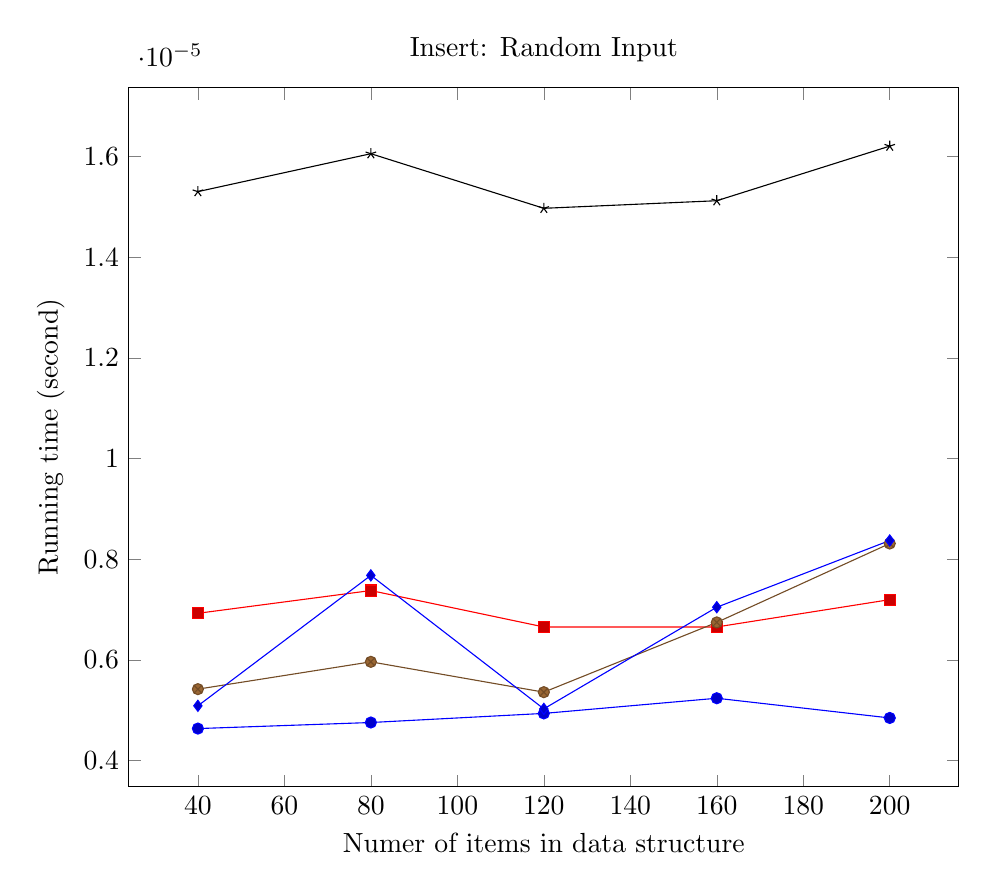
\begin{tikzpicture}
        \begin{axis}[
            xlabel={Numer of items in data structure},
            ylabel={Running time (second)},
            title={Insert: Random Input},
            width=\textwidth
        ]
		\addplot coordinates {
			(40, 4.6381001862272345e-06)
			(80, 4.758570320717581e-06)
			(120, 4.939275522630737e-06)
			(160, 5.240450859389511e-06)
			(200, 4.848922921496524e-06)
		};
		\addplot coordinates {
			(40, 6.927032745451811e-06)
			(80, 7.378795750412337e-06)
			(120, 6.6559749424044415e-06)
			(160, 6.6559749424044415e-06)
			(200, 7.198090548499181e-06)
		};
		\addplot coordinates {
			(40, 5.421156061302667e-06)
			(80, 5.9632716677526785e-06)
			(120, 5.36092099423513e-06)
			(160, 6.746327543183383e-06)
			(200, 8.312439294400065e-06)
		};
		\addplot coordinates {
			(40, 1.5299707106919415e-05)
			(80, 1.6052645448638714e-05)
			(120, 1.4968414236449234e-05)
			(160, 1.5119001905006257e-05)
			(200, 1.6203233117195737e-05)
		};
		\addplot coordinates {
			(40, 5.08986319118776e-06)
			(80, 7.679971087171112e-06)
			(120, 5.029628123764951e-06)
			(160, 7.047502879942158e-06)
			(200, 8.372674361822874e-06)
		};
        \legend{}
        \end{axis}
    \end{tikzpicture}
    \caption{Average of 0 operations, benchmarked every 0, starting at 0.}
\end{figure}